\Subsection{Queue \& Deque}

\begin{problem}\textbf{Maximum of Sliding Window}

    Given an array of integers $a$, there is a sliding window of size $k$ which is moving from the very left of the array to the very right. You can only see the $k$ numbers in the window. Each time the sliding window moves right by one position.

    Return the array that contains maximum elements of each position of the sliding window.

    Time complexity: $O(n)$.

    Space complexity: $O(k)$.\newline

    \underline{Note}: you can solve it on \href{https://leetcode.com/problems/sliding-window-maximum/description/}{LeetCode}

    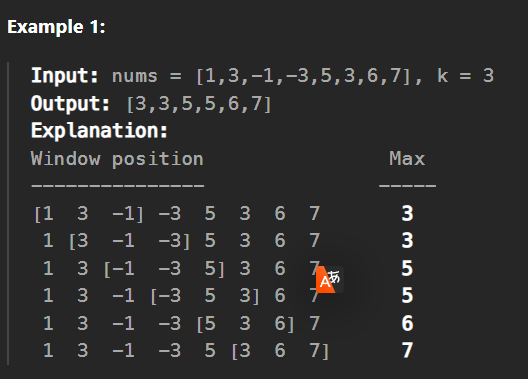
\includegraphics[scale=0.6]{./assets/05-basic-data-structures/1-1.PNG}

    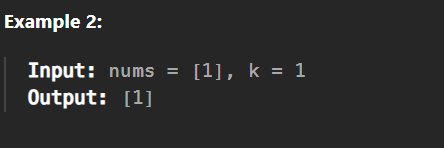
\includegraphics[scale=0.6]{./assets/05-basic-data-structures/1-2.PNG}

\end{problem}


\begin{solution}
    % \textbf{\textnumero 1, Using deque + two pointers}

    % Credits to \textbf{monster0Freason} for a great \href{https://leetcode.com/problems/sliding-window-maximum/solutions/4628595/19-1-approach-1-o-n-python-c-step-by-step-explanation/}{solution}.


    % Let's consider an arbitrary sliding window of size $k$ which contains the following elements:

    % $a_{i_1}, a_{i_2}, ..., a_{i_k}$ ($i_1 < i_2 < ... < i_k$), and this sequence contins $3$ elements $a_{i_n}, a_{i_j}, a_{i_m}$ such that:

    % 1. $i_1 <= i_n < i_j < i_m <= i_k$

    % 2. $a_{i_j} < a_{i_n}$ and $a_{i_j} < a_{i_m}$

    % Notice that for the current sliding window and for the next $m$ sliding windows $a_{i_j}$ will never be a maximum element simply due to the existence of $2$ elements $a_{i_n}$ and $a_{i_m}$ that are greater than $a_{i_j}$ and either of them will be included into the next sliding windows.

    % The above implies that in a sliding window we do not need to keep track of all the elements traversed in $a$ $\implies$ every time we are considering the next element $a_i$ we need to remove all the values kept in the sliding window that are smaller than $a_i$.

    % The above strategy will preserve the invariant over elements in the sliding window $q$: $q_0 \geq q_1 \geq q_3 \geq ... q_{k'}$ (Notice that $k'$ is $\leq$ than $k$).

    % Imagine that we have a queue $q$ that contains on its front (mostleft) part an index of the maximum element for the current sliding window (let's denote it as $x := a[q.front()]$), and we are about to consider next $i$-th element of the array $a$ named $a_i$. There are several cases:

    % 1. $x >= a_i$: then for the sliding window, which is one element forward comparing to the current position, the maximum will remain the same, i.e. $x$.

    % 2. $x < a_i$: then for the next sliding window the maximum element

\end{solution}





\begin{problem}\textbf{Max Value of Equation}

    Given an array $p$ of size $n \leq 10^5$ containing the coordinates of points on a 2D plane, sorted by the $x$-values, i.e. $\{ x_i \}$ form a strictly increasing sequence ($x_i < x_j, \ i < j$), where $p_i = (x_i, y_i)$ ($-10^8 \leq x_i, y_i \leq 10^8$). You are also given an integer $k \leq 2\cdot 10^8$.

    Return the \textbf{maximum value of the equation} $y_i + y_j + |x_i - x_j|$ where $|x_i - x_j| \leq k$ and $0 \leq i < j < n$.

    It is guaranteed that there exists at least one pair of points that satisfy the constraint $|x_i - x_j| \leq k$.

    Time complexity: $O(n)$ or $O(n \cdot \log{n})$.

    Space complexity: $O(k)$.\newline

    \underline{Note}: you can solve it on \href{https://leetcode.com/problems/max-value-of-equation/description/}{LeetCode}

    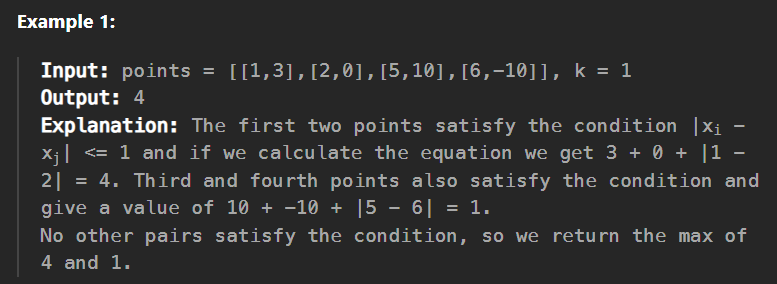
\includegraphics[scale=0.6]{./assets/05-basic-data-structures/2-1.PNG}

    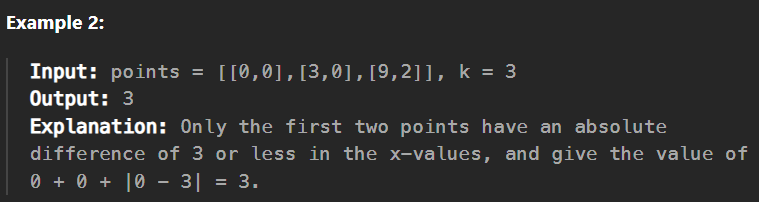
\includegraphics[scale=0.6]{./assets/05-basic-data-structures/2-2.PNG}

\end{problem}


\begin{solution}


\end{solution}